% 4

\chapter{Sviluppo}

Lo sviluppo di un software web come questo richiede l'utilizzo di diverse tecnologie, metodologie e linguaggi di programmazione, anche se non esiste una concreta linea di demarcazione, possiamo distinguere tre specifiche aree di sviluppo:
\begin{itemize}
    \item Database, comprende la traduzione iniziale del modello E/R in uno schema \Gls{sql} operando le opportune normalizzazioni, la creazione di query di ricerca, la creazione di viste e la gestione delle migrazioni dei dati ogniqualvolta una modifica riguarda i dati in produzione.
	\item Back-End, comprende tutto ciò che riguarda la mappatura \Gls{orm} delle tabelle in classi, lo sviluppo della logica del software, ovvero cosa fare con i dati, come trattare quelli ricevuti, cosa restituire all'utente.
	\item Front-End, comprende tutto ciò che riguarda l'interfaccia utente, quindi come presentare i dati passati dal Back-End, la grafica, il template, il typewriting, l’accessibilità e l’usabilità.
	\item Web Service, l'insieme dei software che permettono la comunicazione e lo scambio dati tra la nostra applicazione web e gli altri programmi.
\end{itemize}

% 4.1

\section{Sviluppo del Database}

Prima di scrivere la prima riga di codice è necessario procedere con la definizione dello schema del database, partendo dal modello Entità Relazioni definito in fase di analisi.
A questo punto è necessario scegliere un \Gls{dbms} che implementi il modello, nel nostro caso abbiamo scelto Microsoft SQL Server un \Gls{dbms} relazionale che usa T-SQL come linguaggio di query.
Una volta definito il linguaggio possiamo procedere alla codifica in \Gls{sql} delle tabelle.

\begin{figure}[H]
    \centering
    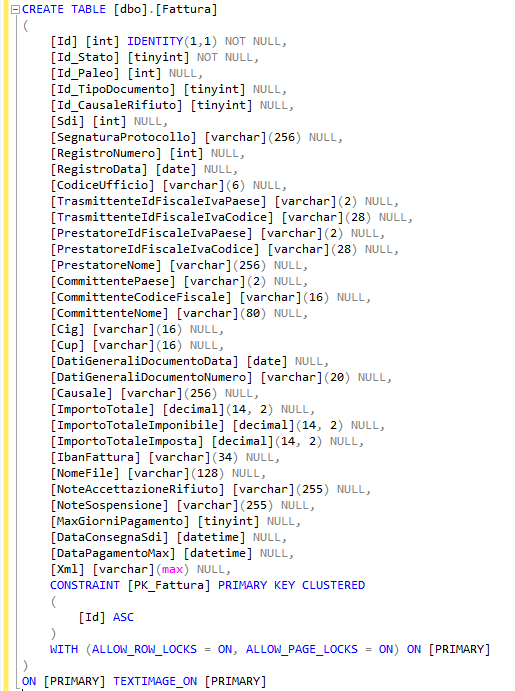
\includegraphics[scale=0.7]{sql-fattura.png}
    \caption{SQL per la creazione della tabella Fattura}
    \label{fig:SqlFattura}
\end{figure}

\begin{figure}[H]
    \centering
    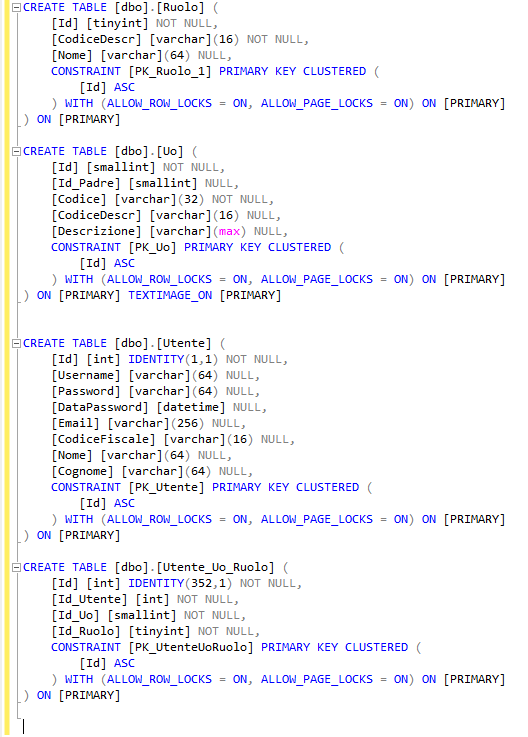
\includegraphics[scale=0.7]{sql-utenteruolouo.png}
    \caption{SQL per la creazione delle tabelle Utente, Ruolo e UO}
    \label{fig:SqlUtenteRuoloUo}
\end{figure}

% 4.2

\section{Sviluppo del Back-End}

Lo sviluppo di Back-End può essere realizzato sia con linguaggi di programmazione lato server come ASP, Java, PHP, sia facendo uso di frameworks come ASP.NET, Spring MVC, Laravel, Django, etc. 

Un framework è una serie di librerie di codice utilizzabili in fase di linking con uno o più linguaggi di programmazione, spesso corredate da una serie di strumenti di supporto allo sviluppo del software, come ad esempio un \Gls{ide}, un debugger o altri strumenti ideati per aumentare la velocità di sviluppo del prodotto finito.

Per realizzare il back-end, è stato scelto di utilizzare il .NET Framework, dato che la maggior parte dei software dell'Ente sono web application in ASP.NET Web Forms, ma si è scelta l'ultima versione del framework allora disponibile e la più recente tecnologia di sviluppo web, ASP.NET MVC.

% 4.2.1

\subsection{.NET Framework}

Il .NET Framework (si pronuncia dot net) è un framework sviluppato da Microsoft eseguibile principalemente su Microsoft Windows.
Include una grande libreria di classi, interfacce e tipi di dato chiamata \Gls{fcl} e garantisce interoperabilità tra i linguaggi di programmazione (ogni linguaggio può usare codice scritto in un altro linguaggio).
I programmi scritti in .NET sono eseguiti in un ambiente software (invece che in un ambiente hardware), conosciuto come \Gls{clr}, una virtual machine che fornisce servizi di sicurezza, gestione della memoria e gestione delle eccezioni.
\Gls{fcl} e \Gls{clr} insieme compongono il .NET Framework.

\begin{figure}[H]
    \centering
    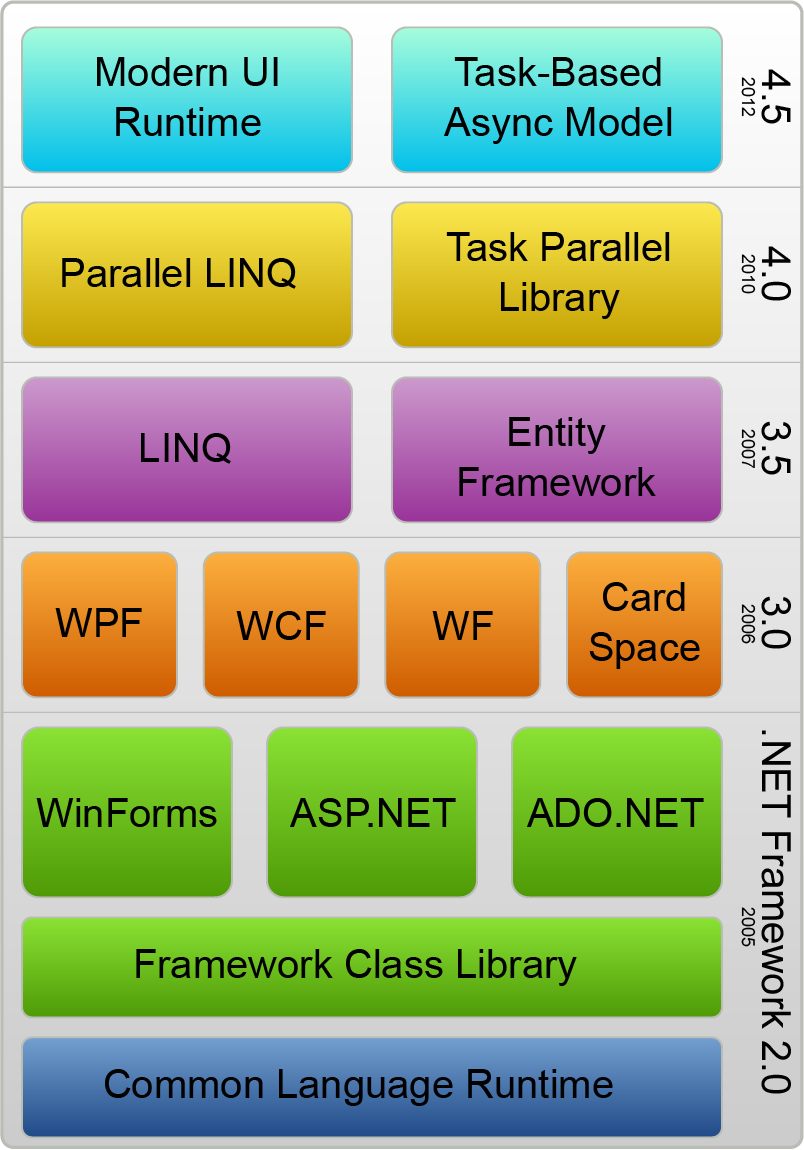
\includegraphics[scale=0.35]{dot-net.png}
    \caption{.NET Framework - Pila dei componenti}
    \label{fig:DotNet}
\end{figure}

Oltre al \Gls{clr} e \Gls{fcl} .NET possiede un insieme di tecnologie per lo sviluppo su diverse piattaforme, alcune di queste tecnologie sono state utilizzate nel nostro progetto, tra le quali:
\begin{itemize}
    \item ASP.NET
    \item Entity Framework
    \item Web API
\end{itemize}

% 4.2.2

\subsection{ASP.NET}

ASP.NET è un insieme di tecnologie software per lo sviluppo di web application e web services, si appoggia sul .NET Framework e offre tre frameworks per la creazione di web application: 
\begin{itemize}
	\item ASP.NET Web Pages, pagine dinamiche dove il markup HTML e il codice sono insieme nello stesso file
	\item Web Forms, che offre una libreria di controlli che incapsulano markup HTML, script javascript e logiche lato server per garantire una gestione ad eventi simile a quella delle applicazioni desktop
	\item ASP.NET MVC, alta separazione delle logiche di controllo, da quelle di presentazione e dai dati grazie al paradigm MVC, tipico anche di altri framework moderni
\end{itemize}

\textbf{ASP.NET MVC} \cite{mvc} fa uso dell'architettura multi-tier chiamata \Gls{mvc} che prevede la separazione del codice in 3 livelli:
\begin{itemize}
    \item Model (Modello), gestisce l'accesso ai dati dell'applicazione
    \item View (Vista), gestisce la visualizzazione dei dati all'utente
    \item Controller (Controllore), gestisce le interazioni dell'utente
\end{itemize}

\begin{figure}[H]
    \centering
    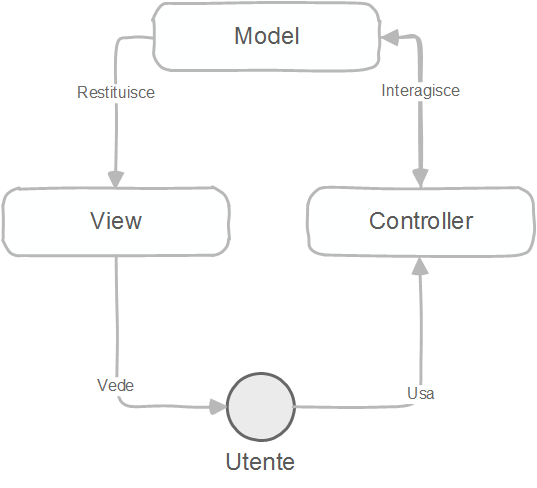
\includegraphics[scale=1]{mvc-pattern.png}
    \caption{Architettura MVC}
    \label{fig:Mvc}
\end{figure}

Il modo in cui questi 3 livelli interagiscono può cambiare da linguaggio a linguaggio, ma nel caso specifico di ASP.NET MVC funziona così:
\begin{enumerate}
    \item l'utente invia una richiesta al browser (può essere una GET o una POST);
    \item la richiesta viene intercettata dal web server (\Gls{iis} nel nostro caso);
    \item il web server fa gestire la richiesta al controller appropriato;
    \item il controller la analizza e decide a quale specifico metodo farla gestire (nel nostro caso i metodi del controller si chiamano Action);
    \item il controller può scegliere se lavorare o meno con il Model, in ogni caso alla fine del metodo ritornerà all'utente una View, cioè una pagina web di risposta.
\end{enumerate}
Nel caso in cui il controller dovesse interfacciarsi con il database chiamerebbe il Model, il quale ha accesso diretto al database e colloquia con esso attraverso query \Gls{sql}.
Di seguito in Figura ~\ref{fig:Action1} vediamo un esempio di Action per la visualizzazione dei Dettagli: tra i parametri del metodo c'è l'ID, passato al metodo tramite URL, e come valore di ritorno c'è la View specifica per Dettagli, a cui viene passato l'oggetto vmFattura.

\begin{figure}[H]
    \centering
    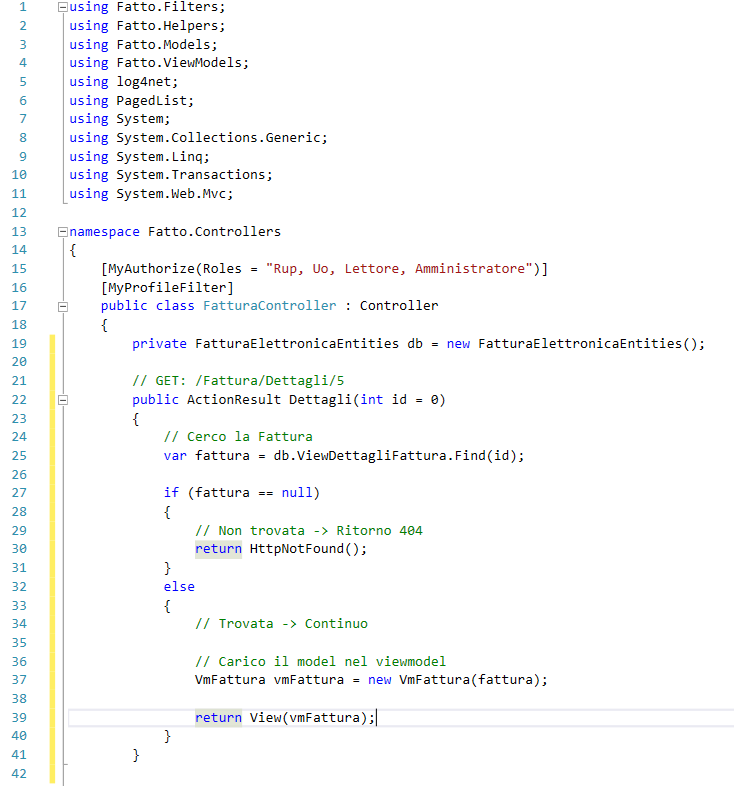
\includegraphics[scale=0.6]{action-1.png}
    \caption{Fattura Controller - Action }
    \label{fig:Action1}
\end{figure}

A volte può essere necessario aggiungere alcuni controlli ricorrenti all'inizio di alcune Actions o sul Controller stesso (in modo che valgano per tutte le Action del Controller), come ad esempio un metodo che controlli se l'utente è autenticato, in quel caso è possibile creare dei Filters o utilizzare quelli di base forniti dal framework (come Authorize).
Nel nostro caso è stato necessario creare un nuovo Filter che ereditasse Authorize, ma che gestisse l'autenticazione Cohesion, richiamando quindi il \Gls{ws} in caso di mancata autenticazione, come in Figura ~\ref{fig:Filter1}.

\begin{figure}[H]
    \centering
    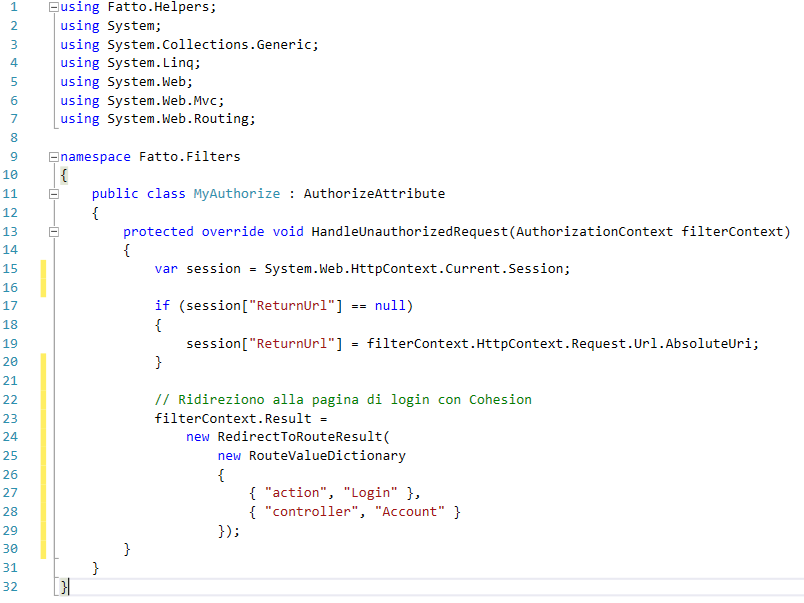
\includegraphics[scale=0.6]{filter-1.png}
    \caption{MyAuthorize Filter}
    \label{fig:Filter1}
\end{figure}

% 4.2.3

\subsection{Entity Framework}

La generazione delle classi del Model e i metodi per accedere al database possono essere gestiti da \Gls{ef}.
Entity Framework è un framework open-source \Gls{orm} per ADO.NET, una parte del .NET Framework: il compito svolto dagli \Gls{orm} è quello di nasconderci il funzionamento di un database relazionale, permettendoci di pensare al nostro modello dei dati come ad un insieme di oggetti.
Mediante l'uso di \Gls{ef} è possibile interrogare il database facendo uso di \Gls{linq}, componente del .NET Framework costituito interamente da "extension methods", ovvero metodi che consentono di estendere le funzionalità di determinati tipi senza dover appositamente definire specifici tipi derivati; esso aggiunge la possibilità di effettuare query su collezioni di dati, con una sintassi simile alla sintassi di SQL oppure simile a quella della programmazione ad oggetti (Lamda Expression).
Entity Framework mette a disposizione tre differenti modalità per interagire con i dati:
\begin{itemize}
    \item Database first, è previsto nel caso in cui il database sia già disponibile, verrà generato in automatico il Data Model che consiste nell'insieme di classi e proprietà che corrispondono alle tabelle ed alle colonne del database. La corrispondenza tra il Data Model così generato e lo schema del database è descritto in formato XML in un file di estensione .edmx. Questo approccio permette modifiche dirette sul database, seguite poi da un'aggiornamento del file edmx.
    \item Model first, consiste nell'uso di uno strumento grafico per la creazione di Data Models chiamato Entity Framework Designer. Analogamente al caso precedente, la corrispondenza tra il database ed il Data Model è descritta mediante un file edmx. Questo approccio non permette modifiche né lato codice né lato database, ma solo tramite lo strumento grafico.
    \item Code first, è un approccio applicabile sia nel caso in cui si disponga già del database, sia in caso contrario. Attraverso la creazione di classi si definiscono le tabelle e loro relazioni, non necessita di un file .edmx e permette di eseguire delle migrazioni di dati da una versione all'altra del database.
\end{itemize}
Nel nostro progetto abbiamo utilizzato l'approccio Database-first.

% 4.3

\newpage

\section{Sviluppo del Front-End}

Per lo sviluppo di un interfaccia utente efficace si deve tener conto di due aspetti oltre a quello tecnico, che sono:
\begin{itemize}
\item Accessibilità
\item Usabilità
\end{itemize}

L'\textbf{usabilità} è un approccio alla progettazione volto a rendere l'interazione tra il prodotto e l'utente migliore sotto i seguenti aspetti:
\begin{itemize}
    \item Efficacia, cioè permettere agli utenti di raggiungere i loro obiettivi in maniera precisa e completa;
    \item Efficienza, cioè l'ottimizzazione delle risorse impiegate;
    \item Soddisfazione, come libertà dal disagio e attitudine positiva con cui gli utenti raggiungono specifici obiettivi attraverso l’uso del prodotto.
\end{itemize}
Nel web, l'usabilità si pone i seguenti obiettivi:
\begin{itemize}
    \item Presentare l'informazione all'utente in modo chiaro e conciso, evitando termini tecnici o specialistici;
    \item Semplificare la struttura del compito;
    \item Offrire all'utente le scelte corrette, in una maniera che risulti ovvia;
    \item Organizzare ogni pagina in modo che l'utente riconosca la posizione e le azioni da compiere;
    \item Eliminare ogni ambiguità relativa alle conseguenze di un'azione (es. fare clic su cancella/rimuovi/compra);
    \item Mettere la cosa più importante nella posizione giusta della pagina web o dell'applicazione web;
    \item Fare in modo che l'utente abbia un rapido feedback ad ogni azione compiuta, ad esempio la comparsa di un messaggio di successo o errore all'invio di dati con una form;
    \item Rendere la grafica accattivante ed interessante dal punto di vista visivo attraverso l'uso di diagrammi, tabelle, sezioni informative e coordinando bene i colori;
    \item Ridurre gli sforzi cognitivi dell'utente.
\end{itemize}
In generale cercare di rendere il sistema il più semplice possibile da usare, in modo da ridurre al minimo gli sforzi sull'utilizzo del mezzo.

L'\textbf{accessibilità} è un aspetto di fontamentale importanza, specialmente per un gestionale web di una \Gls{pa}; il suo scopo è garantire l'accesso alle risorse (prodotti e servizi) da parte di chiunque, siano essi soggetti con disabilità, con scarse competenze informatiche o con dispositivi diversi.
I criteri dell'accessibilità sono quelli delle linee guida del \Gls{w3c} che attraverso una sua sezione denominata \Gls{wai} \cite{w3c-wai} ha definito i linguaggi e le procedure standard per rendere il Web uno strumento realmente democratico e universale.
Queste direttive sono state percepite in Italia con la Legge "Stanca" (Legge 4/2004) che sancisce obblighi e sanzioni per la \Gls{pa} e le aziende appaltate.
In generale i requisiti di accessibilità contenuti nella Legge Stanca e successive modificazioni, contenuti anche in un documento online sul sito del governo \cite{agid-access}, sono i seguenti:
\begin{itemize}
    \item Alternative testuali, obbligatorie per tutte i contenuti non testuali (come immagini, filmati e audio);
    \item Adattabilità, cioè prevedere che i contenuti si adattino a diversi layout in base alla grandezza e al formato dello schermo utente (responsive web design);
    \item Distinguibile, rendere più semplice agli utenti la visione e l'ascolto dei contenuti, separando i contenuti in primo piano dallo sfondo;
    \item Accessibile da tastiera, cioè garantire una buona navigabilità prevedendo un percorso di TAB;
    \item Colori, il contrasto tra le scritte e lo sfondo deve essere chiaro, ma non si devono usare colori discordanti tra loro o lampeggianti che possano causare crisi epilettiche;
    \item Navigabile, fornire una struttura del sito chiara, dove l'utente possa orientarsi e raggiungire qualsiasi sezione attraverso links;
    \item Assistenza per l'inserimento, fornire gli aiuti e le spiegazioni necessarie affinché l'utente sia in grado di compilare correttamente le form del sito;
    \item Compatibilità, il sito deve essere accessibile da tutte le piattaforme e deve utilizzare tecnologie standard.
\end{itemize}

% 4.3.1

\subsection{Tecnologie usate nello sviluppo del front-end}

Mentre per lo sviluppo del back-end abbiamo a disposizione una gran quantità di tecnologie concorrenti per svolgere lo stesso compito, per il front-end le tecnologie di base sono sempre le stesse: \Gls{html}, \Gls{css} e JavaScript.

\textbf{\Gls{html}} \cite{w3c-html} è un linguaggio di markup per le pagine web i cui standard sono definiti dal \Gls{w3c} e serve per descrivere il contenuto di una pagina web, sia testuale che multimediale, attraverso dei tag.
Sebbene il linguaggio sia in grado di definire anche regole di formattazione come la centratura del testo o la dimensione dei caratteri, il suo scopo primario è quello di descrivere i contenuti e il loro significato semantico, attraverso l'uso dei tag appropriati (ad esempio \textless p\textgreater  per i paragrafi, \textless h1\textgreater  per un titolo di primo livello, \textless  address\textgreater  per informazioni relative ad un indirizzo, etc.).
Attualmente la versione più recente delle specifiche è chiamata HTML 5 e comporta rispetto alle precedenti versioni l'aggiunta di alcuni tag per gli elementi multimediali, il miglioramento i controlli di input per le form, il controllo della geolocalizzazione e l'intruduzione dello Web Storage come alternativa ai cookies.

\textbf{\Gls{css}} \cite{w3c-css} è il linguaggio usato per definire il layout (impaginazione), la formattazione del testo e l'aspetto grafico in generale; può essere definito sia all'interno della pagina \Gls{html} che all'esterno come file a sé stante, che è generalamente la scelta migliore.
Nel nostro caso sono state usate alcune delle proprietà più recenti del linguaggio come la box-shadow o la border-radius appartenenti alle specifiche CSS 3.
Per mantenere la compatibilità tra i differenti browser (e nei limiti del possibile anche con le versioni più vecchie degli stessi) sono state applicate ad ogni proprietà CSS 3 delle tecniche di cross-browsing, cioè la riscrittura della stessa proprietà in modi differenti, vedi figure ~\ref{fig:Css3Shadow} e ~\ref{fig:Css3Radius}.

\begin{figure}[H]
    \centering
    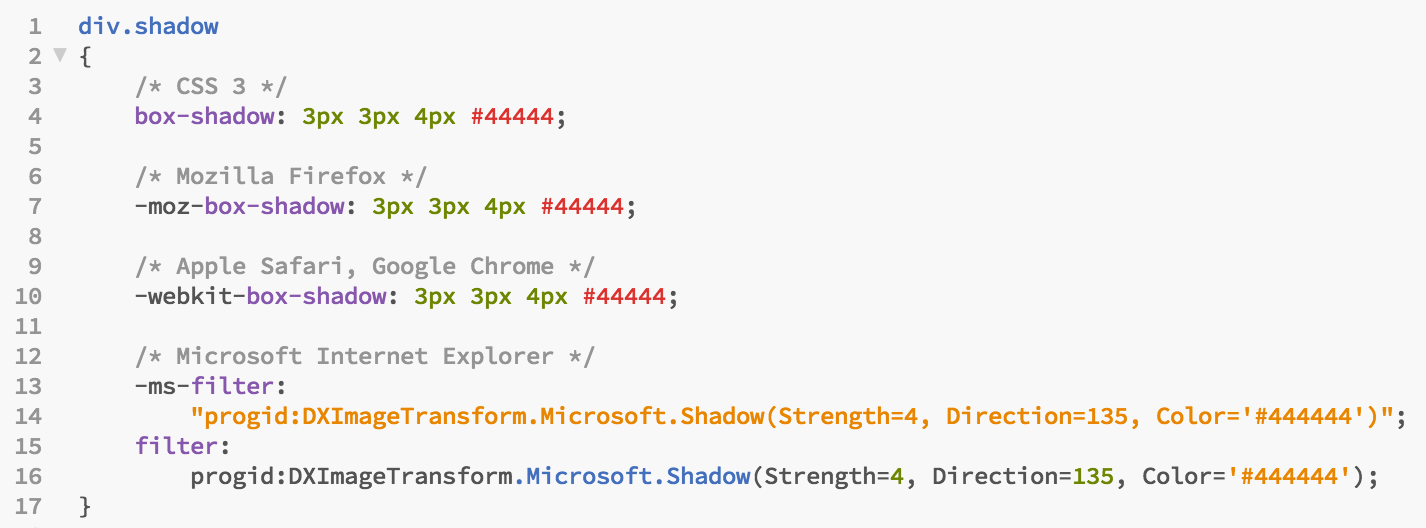
\includegraphics[scale=0.5]{css3-1.png}
    \caption{CSS 3 text-shadow cross-browser}
    \label{fig:Css3Shadow}
\end{figure}

\begin{figure}[H]
    \centering
    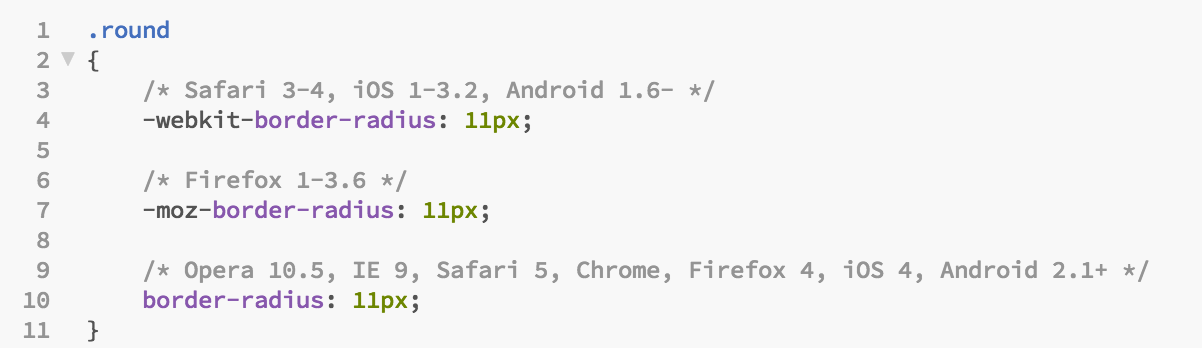
\includegraphics[scale=0.5]{css3-2.png}
    \caption{CSS 3 border-radius cross-browser}
    \label{fig:Css3Radius}
\end{figure}

\textbf{JavaScript} \cite{javascript} è un linguaggio di scripting adatto per creare effetti dinamici interattivi basati su eventi, come il click di un bottone, la selezione di una voce da una tendina, la pressione di un tasto o il caricamento di una pagina.
Anche se con il javascript è possibile creare applicazioni vere e proprie si deve sempre tener conto che è un linguaggio accessorio, ovvero c'è la possibilità per l'utente di disabilitarlo, specialmente nel caso si abbia delle disabilità o dei problemi di visualizzazione.
Pertanto nessuna funzionalità deve contare unicamente su javascript per funzionare, ma il suo uso è comunque consigliato per aumentare l'esperienza utente (quegli obiettivi dell'usabilità esposti sopra) ad esempio prevedendo dei messaggi di errore nel caso si inseriscano dei valori errati nei campi, o un calendario all'immissione di un campo data, o anche per sostituire delle proprietà del CSS 3 nel caso il browser dell'utente non la supporti (i cosiddetti polyfill).

\textbf{jQuery} \cite{jquery} è una libreria Javascript molto diffusa il cui scopo è semplificare la selezione, la gestione e la manipolazione degli eventi, mantenendo però anche la possibilità di utilizzare il linguaggio nella vecchia maniera.
L'uso di jQuery non aggiunge quindi nessuna funzionalità, rende solamente più semplice l'utilizzo del linguaggio e quindi più elevata la produttività del programmatore, non a caso il suo motto è "Write less, do more", anch'essa è stata inclusa nella nostra applicazione web e gli script personalizzati fanno tutti riferimento alla sua sintassi.

\textbf{\Gls{ajax}} è un'altra tecnologia molto importante per migliorare l'esperienza utente, perché permette di aggiornare il contenuto di una pagina dinamicamente senza effettuare il "refresh" e quindi caricando solo le informazioni necessarie, anziché tutta la pagina.
Si tratta, più che di un nuovo linguaggio, di un insieme di tecniche che fanno uso delle tecnologie sopra descritte, quindi JavaScript per inviare le richieste asincrone e XML o JSON per ricevere le risposte dal server sottoforma di oggetti.
Questa tecnica è stata utilizzata nella nostra applicazione web nella fase di autenticazione post-Cohesion, dove viene richiesto all'utente di scegliere un ruolo da una tendina e automaticamente sulla base di questa scelta viene popolata la tendina delle \Gls{uo} riferite a quel ruolo.
Un altro utilizzo è nella pagina di inserimento di un nuovo utente, dove a seguito della digitazione di almeno 3 caratteri in una casella di testo, compare un menù di autocomplete che suggerisce i possibili nomi degli utenti cercati.

\textbf{Razor} \cite{razor} infine, è un linguaggio di programmazione lato server, specifico del framework ASP.NET MVC, ma è stato incluso in questa sezione perché serve a descrivere, insieme all'HTML, il contenuto di una View.
Una View che contiene codice Razor sarà un file di tipo .cshtml (nel caso il linguaggio lato server utilizzato sia il C\#).
Questo linguaggio può utilizzare molte delle classi del framework, semplicemente includendo il namespace nella pagina, ma il suo scopo principale è quello di posizionare gli elementi del Model nella View, passati dal Controller, eventualmente anche iterando una Collection affinché venga stampata a schermo una serie di elementi per ogni elemento della Collection, come in Figura ~\ref{fig:Razor}.

\begin{figure}[H]
    \centering
    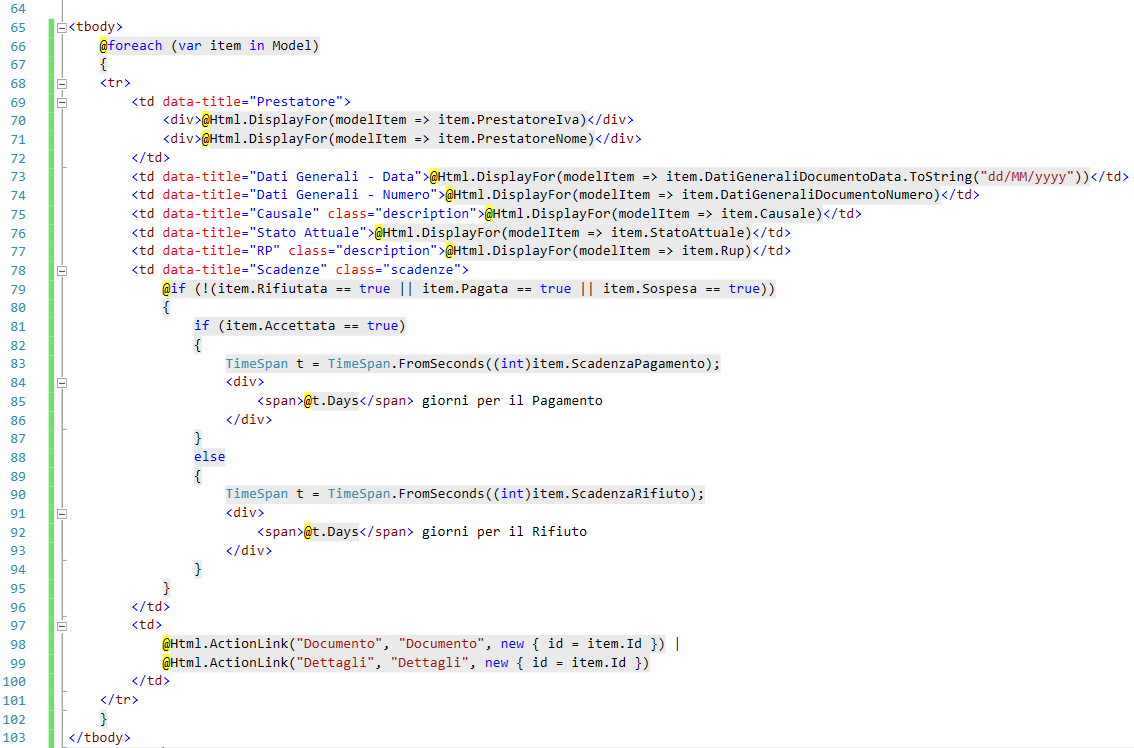
\includegraphics[scale=0.5]{razor-1.png}
    \caption{Esempio di codice Razor per la stampa degli elementi di una collection come righe di una tabella HTML}
    \label{fig:Razor}
\end{figure}

% 4.4

\section{Sviluppo dei Web Service}

Lo scambio dati tra diversi programmi può avvenire sostanzialmente in diversi modi:
\begin{itemize}
    \item Salvando dati in un database comune
    \item Salvando dati sottoforma di file in una locazione di memoria comune
    \item Scambiandosi i dati tra applicazione attraverso web service
\end{itemize}
La soluzione più utilizzata, e nel nostro caso l'unica percorribile, è quella di esporre web service o utilizzare quelli messi a disposizione dalle altre applicazioni web.

% 4.4.1

\subsection{REST e SOAP}

Un web service è un metodo di comunicazione tra due applicazioni o dispositivi elettronici in rete.
I web service possono essere di due tipi:
\begin{itemize}
    \item \Gls{soap}
    \item \Gls{rest}
\end{itemize}

\textbf{\Gls{soap}} \cite{soap} definisce un protocollo (insieme di regole) tra le due applicazioni per la comunicazione mediante lo scambio di messaggi \Gls{xml}.
Tale protocollo è descritto da un file chiamato \Gls{wsdl} che descrive i tipi di dato e i metodi che un client può richiamare per utilizzare il web service.
\Gls{soap} utilizza \Gls{http} come protocollo per lo scambio di messaggi, ma non è limitato né vincolato ad esso, dal momento che può benissimo usare altri protocolli, come \Gls{smtp}.
%A differenza di \Gls{http}, le specifiche di \Gls{soap} non affrontano argomenti come la sicurezza o l’indirizzamento, per i quali sono stati definiti standard a parte, nello specifico WS-Security e WS-Addressing.

\textbf{\Gls{rest}} descrive un insieme di principi architetturali con i quali i dati possono essere trasmessi attraverso un'interfaccia standard (come \Gls{http}).
Alla base di un servizio RESTful c'è il concetto di risorsa, cioè un oggetto o una collection, a cui il client può accedere tramite un \Gls{uri}.
I metodi con i quali il client può accedere sono quelli del protocollo \Gls{http} (GET, POST, PUT, DELETE e HEAD) e il content-type è definito da chi espone il web service, tipicamente \Gls{json} o \Gls{xml}.

% 4.4.2

\subsection{Web API 2}

ASP.NET Web API \cite{web-api} è un framework che rende semplice la costruzione di web service \Gls{http} in grado di raggiungere un gran numero di client, tra i quali browser e dispositivi mobili.
È la piattaforma ideale per creare applicazioni \Gls{rest} in \Gls{net}, in quanto utilizza lo stesso modello architetturale di ASP.NET MVC.
Per creare un nuovo Web Service bisogna creare un controller riferito a una specifica risorsa, ad esempio la fattura, e creare la Action corrispondente al metodo con il quale si vuole consentire l'accesso alla risorsa, ad esempio GET.
Come parametri del metodo Action si possono indicare parametri singoli, come ad esempio l'ID che costituirà l'\Gls{uri} della richiesta, oppure oggetti che andranno a comporre il payload (tipicamente di una richiesta POST o PUT).
Attraverso i filter è possibile gestire delle politiche di sicurezza come la Basic Authentication.
La versione utilizzata per i web service del nostro software è chiamata Web API 2.
Di seguito in Figura ~\ref{fig:Api1} vediamo parte del \Gls{ws} chiamato da \Gls{imm} per aggiornare lo stato fattura quando arriva dallo \Gls{sdi} la notifica di accettazione per decorrenza termini oppure la notifica di scarto.

\begin{figure}[H]
    \centering
    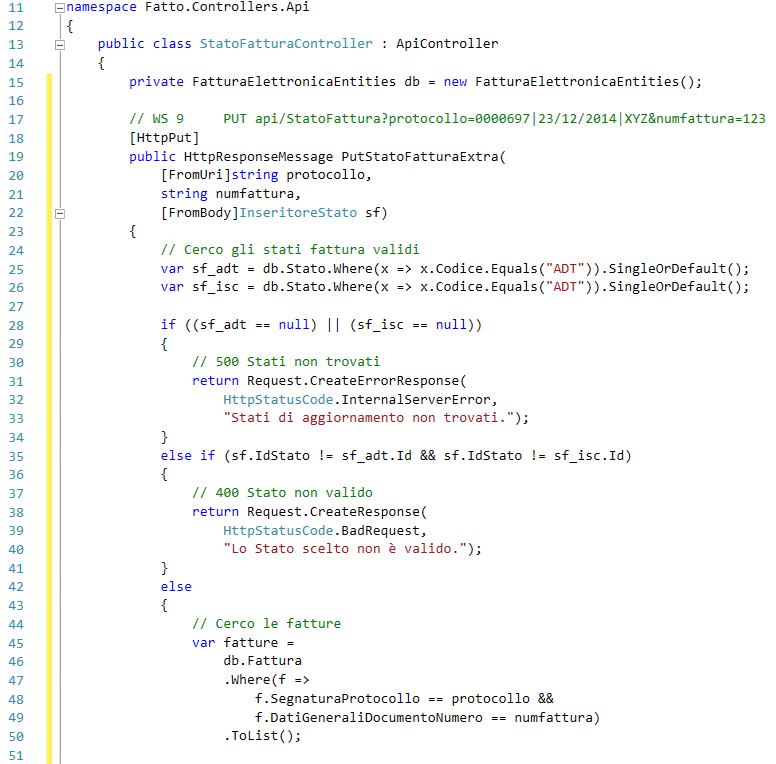
\includegraphics[scale=0.6]{api-1.png}
    \caption{StatoFattura API Controller - PUT Stato }
    \label{fig:Api1}
\end{figure}